\documentclass[../main.tex]{subfiles}
\begin{document}


\noindent \textbf{Example:}
\noindent Let $E$ be a set, $\left\{ 1, 2, 3 \right\}$ then:\\
\noindent Show there are exactly eight non-isomorphic matroids on E. 
 Along with the corresponding Graph of each matroid. This confirms to us the value in the previous table for $n=3.$
    
    
\noindent\TheSolution
\hspace*{10px} 
  
\[ \{ \emptyset  \} \]  
  

\begin{tikzpicture}
  [scale=.8,auto=left,every node/.style={circle,fill=blue!20}]
  \node (n1) at (11,8) {};

\end{tikzpicture}

\noindent\rule{12cm}{0.4pt}
\vspace{10px}

\[  \left\{ \left\{ \emptyset \right\} , \left\{ 1 \right\} \right\} \cong \left\{ \left\{ \emptyset \right\} , \left\{ 2 \right\} \right\} \cong \left\{ \left\{ \emptyset \right\} , \left\{ 3 \right\} \right\} \]   
 
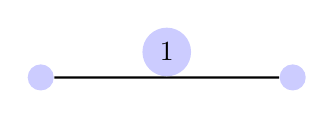
\begin{tikzpicture}
  [scale=.8,auto=left,every node/.style={circle,fill=blue!20}]
  \node (n1) at (11,8) {};
  \node (n2) at (15,8) {};

  \path[draw,thick]
     (n1) edge node {1} (n2);
    
\end{tikzpicture}

\noindent\rule{12cm}{0.4pt}


\[ \left\{ \left\{ \emptyset \right\} , \left\{ 1 \right\},\left\{ 2 \right\} , \left\{ 1, 2 \right\} \right\} \cong  \left\{ \left\{ \emptyset \right\} , \left\{ 1 \right\}, \left\{ 3 \right\} , \left\{ 1, 3 \right\} \right\} \cong  \left\{ \left\{ \emptyset \right\} , \left\{ 2 \right\}, \left\{ 3 \right\} , \left\{ 2, 3 \right\} \right\} \] 
 
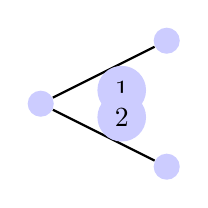
\begin{tikzpicture}
  [scale=.8,auto=left,every node/.style={circle,fill=blue!20}]
  \node (n1) at (11,7) {};
  \node (n2) at (9,6) {};
  \node (n3) at (11,5) {};

  \path[draw,thick]
     (n1) edge node {1} (n2)
     (n2) edge node {2} (n3);
 
\end{tikzpicture}

\noindent\rule{12cm}{0.4pt}


 \[  \left\{ \left\{ \emptyset \right\} , \left\{ 1 \right\}, \left\{ 2 \right\} \right\} \]


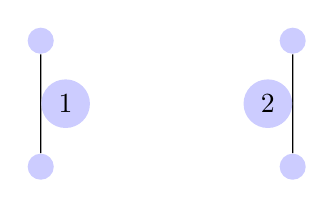
\begin{tikzpicture}
  [scale=.8,auto=left,every node/.style={circle,fill=blue!20}]
  \node (n1) at (5,8) {};
  \node (n2) at (5,6) {};
  \node (n3) at (9,6) {};
  \node (n4) at (9,8) {};

  \path[draw]
     (n1) edge node {1} (n2)
     (n3) edge node {2} (n4);
\end{tikzpicture}

\noindent\rule{12cm}{0.4pt}
\vspace{35px}
  \[  \left\{ \left\{ \emptyset \right\} , \left\{ 1 \right\}, \left\{ 2 \right\}, \left\{ 3 \right\} \right\}  \]

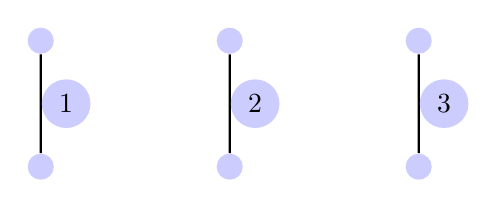
\begin{tikzpicture}
  [scale=.8,auto=left,every node/.style={circle,fill=blue!20}]
  \node (n6) at (11,8) {};
  \node (n4) at (8,8) {};
  \node (n5) at (11,10) {};
  \node (n1) at (5,10) {};
  \node (n2) at (5,8) {};
  \node (n3) at (8,10) {};

  \path[draw,thick]
     (n1) edge node {1} (n2)
     (n3) edge node {2} (n4)
     (n5) edge node {3} (n6);
\end{tikzpicture}

\noindent\rule{12cm}{0.4pt}
\vspace{10px}

 \[  \left\{ \left\{ \emptyset \right\} , \left\{ 1 \right\}, \left\{ 2 \right\}, \left\{ 3 \right\}, \left\{ 1, 2 \right\}, \left\{ 2, 3 \right\} \right\}  \]
 
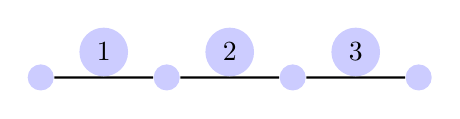
\begin{tikzpicture}
  [scale=.8,auto=left,every node/.style={circle,fill=blue!20}]

  \node (n1) at (5,8) {};
  \node (n2) at (7,8) {};
  \node (n3) at (9,8) {};
  \node (n4) at (11,8) {};

  \path[draw,thick]
     (n1) edge node {1} (n2)
     (n2) edge node {2} (n3)
     (n3) edge node {3} (n4);
    
\end{tikzpicture}

\noindent\rule{12cm}{0.4pt}

\[  \left\{ \left\{ \emptyset \right\} , \left\{ 1 \right\}, \left\{ 2 \right\}, \left\{ 3 \right\}, \left\{ 1, 2 \right\}, \left\{ 1, 3 \right\} , \left\{ 2, 3 \right\} \right\}  \]

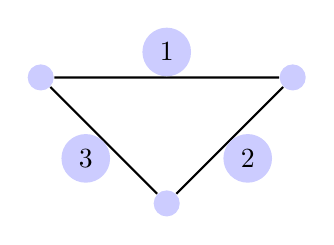
\begin{tikzpicture}
  [scale=.8,auto=left,every node/.style={circle,fill=blue!20}]

  \node (n1) at (5,8) {};
  \node (n2) at (9,8) {};
  \node (n3) at (7,6) {};

  \path[draw,thick]
     (n1) edge node {1} (n2)
     (n2) edge node {2} (n3)
     (n3) edge node {3} (n1);
\end{tikzpicture}

\noindent\rule{12cm}{0.4pt}
\vspace{5px}

  
  \[  \left\{ \left\{ \emptyset \right\} , \left\{ 1 \right\}, \left\{ 2 \right\}, \left\{ 3 \right\}, \left\{ 1, 2 \right\}, \left\{ 1, 3 \right\} , \left\{ 2, 3 \right\} , \left\{ 1, 2, 3 \right\} \right\}  \]
 \begin{minipage}{.2\textwidth}  
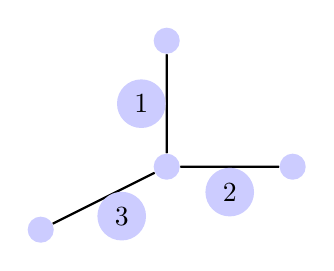
\begin{tikzpicture}
  [scale=.8,auto=left,every node/.style={circle,fill=blue!20}]

  \node (n1) at (10,6) {};
  \node (n2) at (8,6) {};
  \node (n3) at (6,5) {};
  \node (n4) at (8,8) {};
  
  \foreach \from/\to in {n1/n2,n2/n3,n2/n4}
    \draw (\from) -- (\to);
  \path[draw,thick]
     (n1) edge node {2} (n2)
     (n2) edge node {3} (n3)
     (n2) edge node {1} (n4);
\end{tikzpicture}
\end{minipage}

\hspace{4cm}

\begin{minipage}{.2\textwidth}


\end{minipage}
\end{document}